% Chapter 3
% Roberto Masocco <robmasocco@gmail.com>
% September 20, 2021

\chapter[Caso di studio: drone autonomo]{Caso di studio: drone autonomo}
\label{chap:Chapter3}
\doublespacing
\fontsize{14}{14}\selectfont
\indent A seguito della discussione portata a termine nei capitoli precedenti circa le nuove soluzioni hardware e software da impiegare per la costruzione di apparati robotici, verrà ora descritto un caso di studio pratico con cui si dimostreranno la validità e l'efficacia di tali strumenti: un drone volante automatico.\\
I task che tale sistema deve svolgere, oltre naturalmente a quelli inerenti il volo in sé, sono specificati nelle regole dell'edizione 2021 del Drone Contest indetto da Leonardo S.p.A. e tenutosi presso la Divisione Velivoli di Leonardo in Corso Francia, Torino. Il prototipo è stato presentato in tale occasione come la proposta del team Asgard Flight Group dell'Università di Roma "Tor Vergata". Il progetto ha coinvolto in tutto cinque tra tesisti e dottorandi afferenti al Dipartimento di Ingegneria Civile e Ingegneria Informatica, i quali sono citati all'inizio di questa Tesi assieme ai loro ruoli e ad un sentito e personale ringraziamento, sotto la supervisione del Prof. Daniele Carnevale. Le regole dell'edizione 2021 del Contest, che costituiscono gli obiettivi operativi del drone, possono essere riassunti come segue:
\begin{itemize}
    \item il drone deve essere in grado di decollare, volare e atterrare autonomamente, orientandosi all'interno di un ambiente indoor di cui è nota a priori la conformazione e la posizione delle piazzole di decollo e atterraggio;
    \item inizialmente il drone deve esplorare l'ambiente, cercando ed individuando dei target mobili costituiti da robot di tipo Roomba che montano un landmark ArUco;
    \item sono noti solo alcuni dei landmark montati sui robot, dunque quando il drone ne individuasse uno sconosciuto, dovrà scattare ed inviare delle fotografie di esso ad una \emph{Ground Control Station} controllata da un operatore;
    \item sulla base di una stringa di punteggi segnata vicino al landmark del robot, dovrà essere decisa una sequenza di atterraggi sulle varie piazzole;
    \item una volta trasmessa la sequenza al drone, esso dovrà eseguire i vari atterraggi, riconoscendo le piazzole sapendone la posizione nella mappa e rilevando i landmark ArUco dipinti su di esse;
    \item durante tutta la durata del volo deve essere possibile inserire il controllo manuale, per ragioni di sicurezza;
\end{itemize}
Per brevità sono stati tralasciati dei dettagli del regolamento inerenti il solo funzionamento della gara. L'obiettivo finale del Contest è chiaramente la massimizzazione del punteggio ottenuto con gli atterraggi, resa non banale dalla presenza nella mappa di ostacoli, rialzi e zone a bassa visibilità.\\
Nel resto di questo capitolo si descriverà più nel dettaglio il robot, partendo dall'hardware e passando poi al software, da quello di più basso livello fino alle logiche di supervisione e comunicazione con GCS ed operatori.\\
Il prototipo realizzato, assieme ad un esempio di landmark ArUco, sono ritratti in Figura \ref{fig:drone}.

\begin{figure}
    \centering
    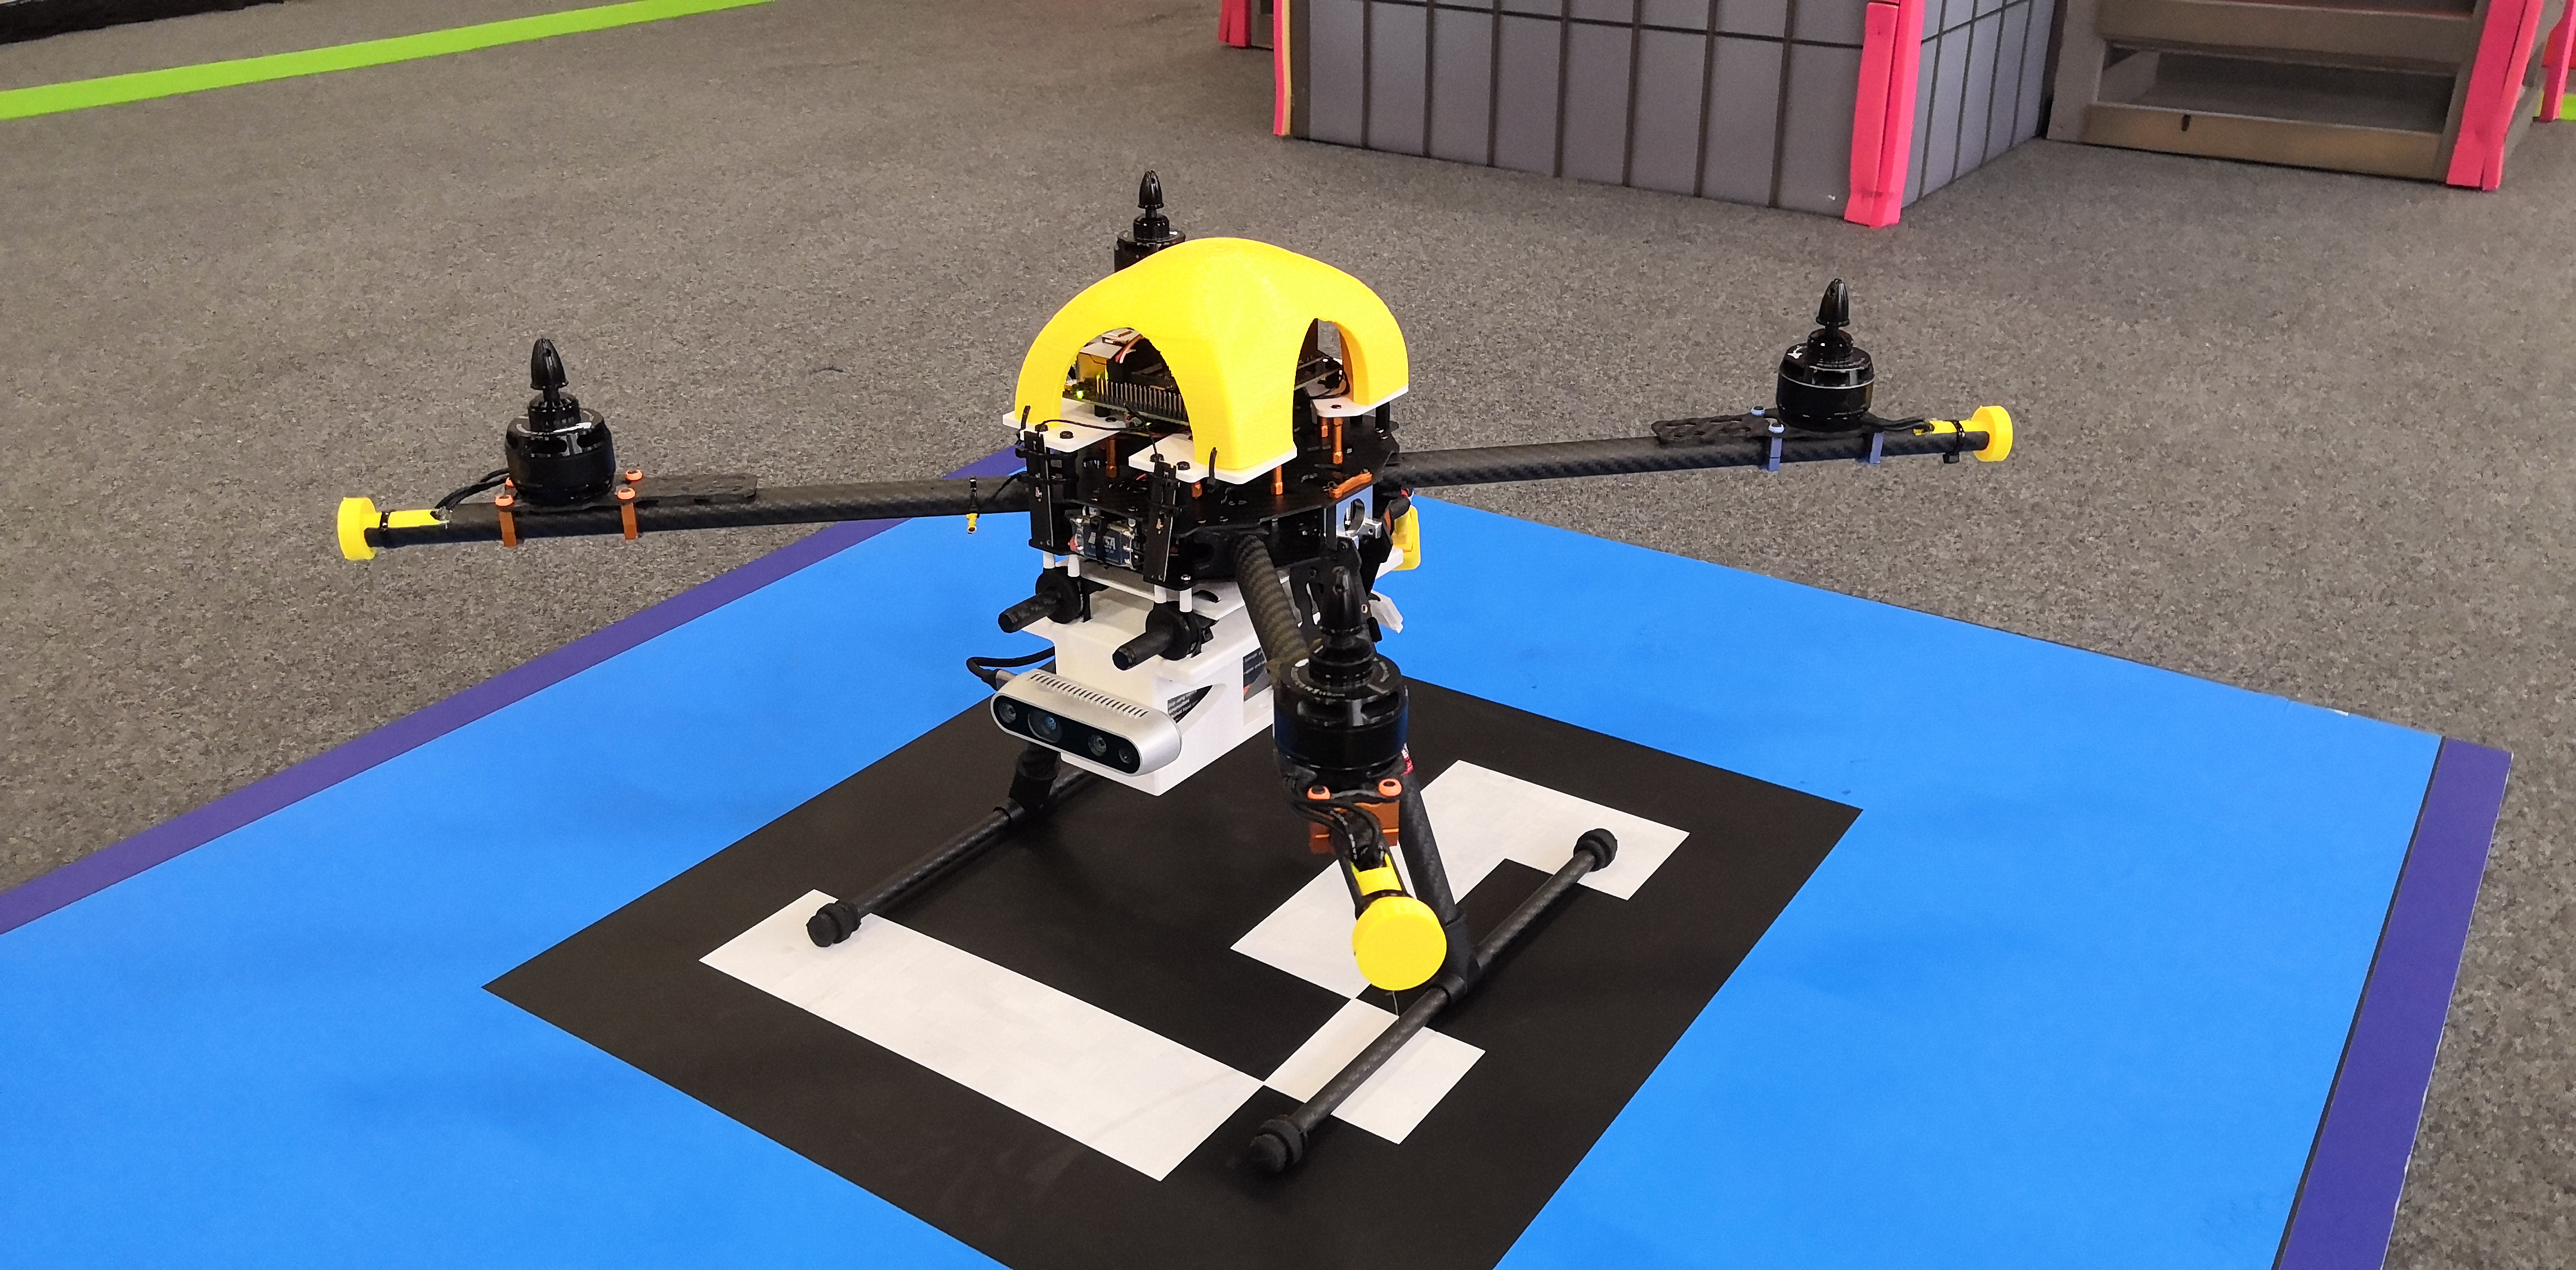
\includegraphics[width=0.9\textwidth]{figs/chapter3/drone_aruco.jpg}
    \caption{Prototipo del drone con le eliche rimosse su una piazzola del campo.}
    \label{fig:drone}
\end{figure}
\clearpage

\newsection{Hardware}
\newsubsection{Frame e motori}
\indent La primissima decisione progettuale ha riguardato la scelta del \emph{frame}, inteso come struttura portante, su cui montare le varie parti. Nell'economia di un drone volante, in special modo autonomo quindi in grado di stabilizzarsi da solo grazie al feedback di vari sensori di bordo, tale struttura deve essere il più leggera e rigida possibile: il primo requisito riguarda naturalmente le prestazioni, l'autonomia e la controllabilità, mentre il secondo ha risvolti sull'accuratezza delle misure di accelerometri e giroscopi. È infatti comune rilevare durante il volo, mediante uno spettrogramma ricavato dai campioni degli accelerometri, delle vibrazioni dovute a vari fattori. Un esempio è mostrato in Figura \ref{fig:flightspec}, relativo ad una prova di volo automatico in pattugliamento. Prendendola ad esempio, si possono notare dei contributi frequenziali predominanti intorno ai 90 Hz, correlati ad altri precedenti nello spettro e di ampiezza minore: sono le armoniche dei motori. Tali vibrazioni non possono naturalmente essere eliminate, e vanno filtrate e reiezionate dal sistema di controllo e stabilizzazione angolare. Alla fine dello spettrogramma (a circa 6:40) si nota quello che sembra un breve urto, che corrisponde al contatto col suolo in fase di atterraggio, in questo caso preciso e privo di rimbalzo. Eventuali altri contributi significativi, in questo caso assenti, sarebbero indice di problemi meccanici o tarature sbagliate del sistema di controllo.\\
Avendo a che fare con questo genere di prototipo però, è necessario anche uno spazio sufficiente ad ospitare i sistemi elettronici, i sensori e le batterie. Per questo la scelta è ricaduta sul frame Tarot 650, realizzato in carbonio e dotato di una piattaforma centrale sufficientemente ampia da permettere il montaggio dell'elettronica di bordo ricavando due livelli superiori e di un pacco batterie in basso. L'intera struttura è stata pensata avendo cura di spostare il meno possibile lungo la verticale il centro di massa aggiungendo carico al frame: montando la batteria in basso questo tende naturalmente a scendere, imprimendo al sistema un comportamento indesiderato simile a quello di un pendolo composto, caratterizzato da oscillazioni difficili da contrastare. A seguito delle diverse prove e dei vari incidenti di percorso, sono state aggiunte dei pezzi volti a irrobustire i punti più fragili e ridurre ancor di più le vibrazioni. Le ulteriori parti meccaniche necessarie sono state modellate con strumenti CAD e stampate in 3D in PLA e TPU: degli esempi particolarmente rilevanti sono mostrati nelle Figure \ref{fig:batpack}, \ref{fig:frontcam}, \ref{fig:canopy}, \ref{fig:triangle}.\\
Per fornire spinta sono stati montati quattro motori brushless T-Motor U3 da 700 W e 700 rpm/V, dotati di eliche da 12 pollici. Essi sono pilotati dal controllore di volo mediante delle ESC\footnote{Electronic Speed Controller.} F35A BLHeli\_32 digitali a 32 bit con protocollo DShot, configurato per trasmissione a 1200 kpbs. Tale protocollo è particolarmente indicato per la trasmissione di comandi agli attuatori dei droni in quanto garantisce bassissima latenza, robustezza agli errori sui bit, e permette di comunicare direttamente con le ESC per configurarle, consentendo ad esempio di impostare il verso di rotazione dei motori senza dover dissaldarne i cavi per invertire le polarità.

\begin{figure}
    \centering
    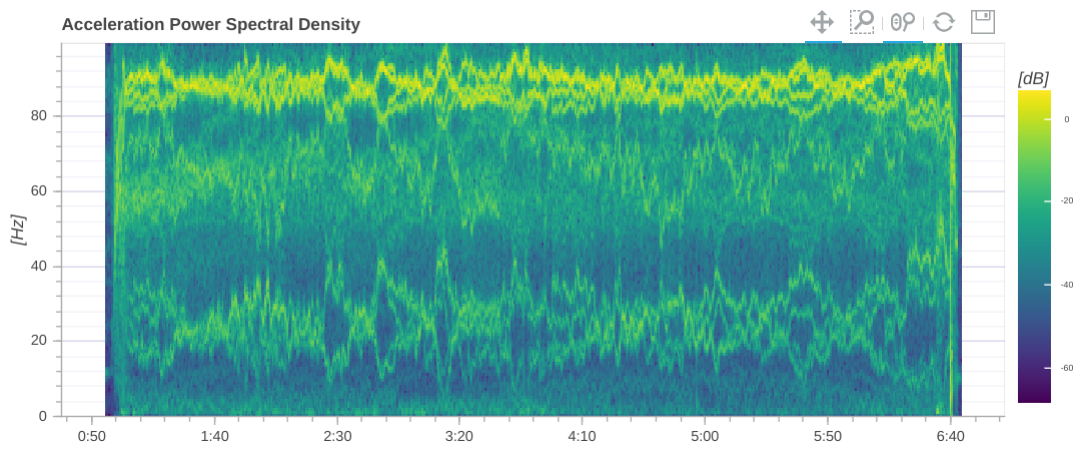
\includegraphics[width=0.9\textwidth]{figs/chapter3/flight_spectro.png}
    \caption{Esempio di spettrogramma ricavato dai dati di un volo automatico.}
    \label{fig:flightspec}
\end{figure}

\begin{figure}
    \centering
    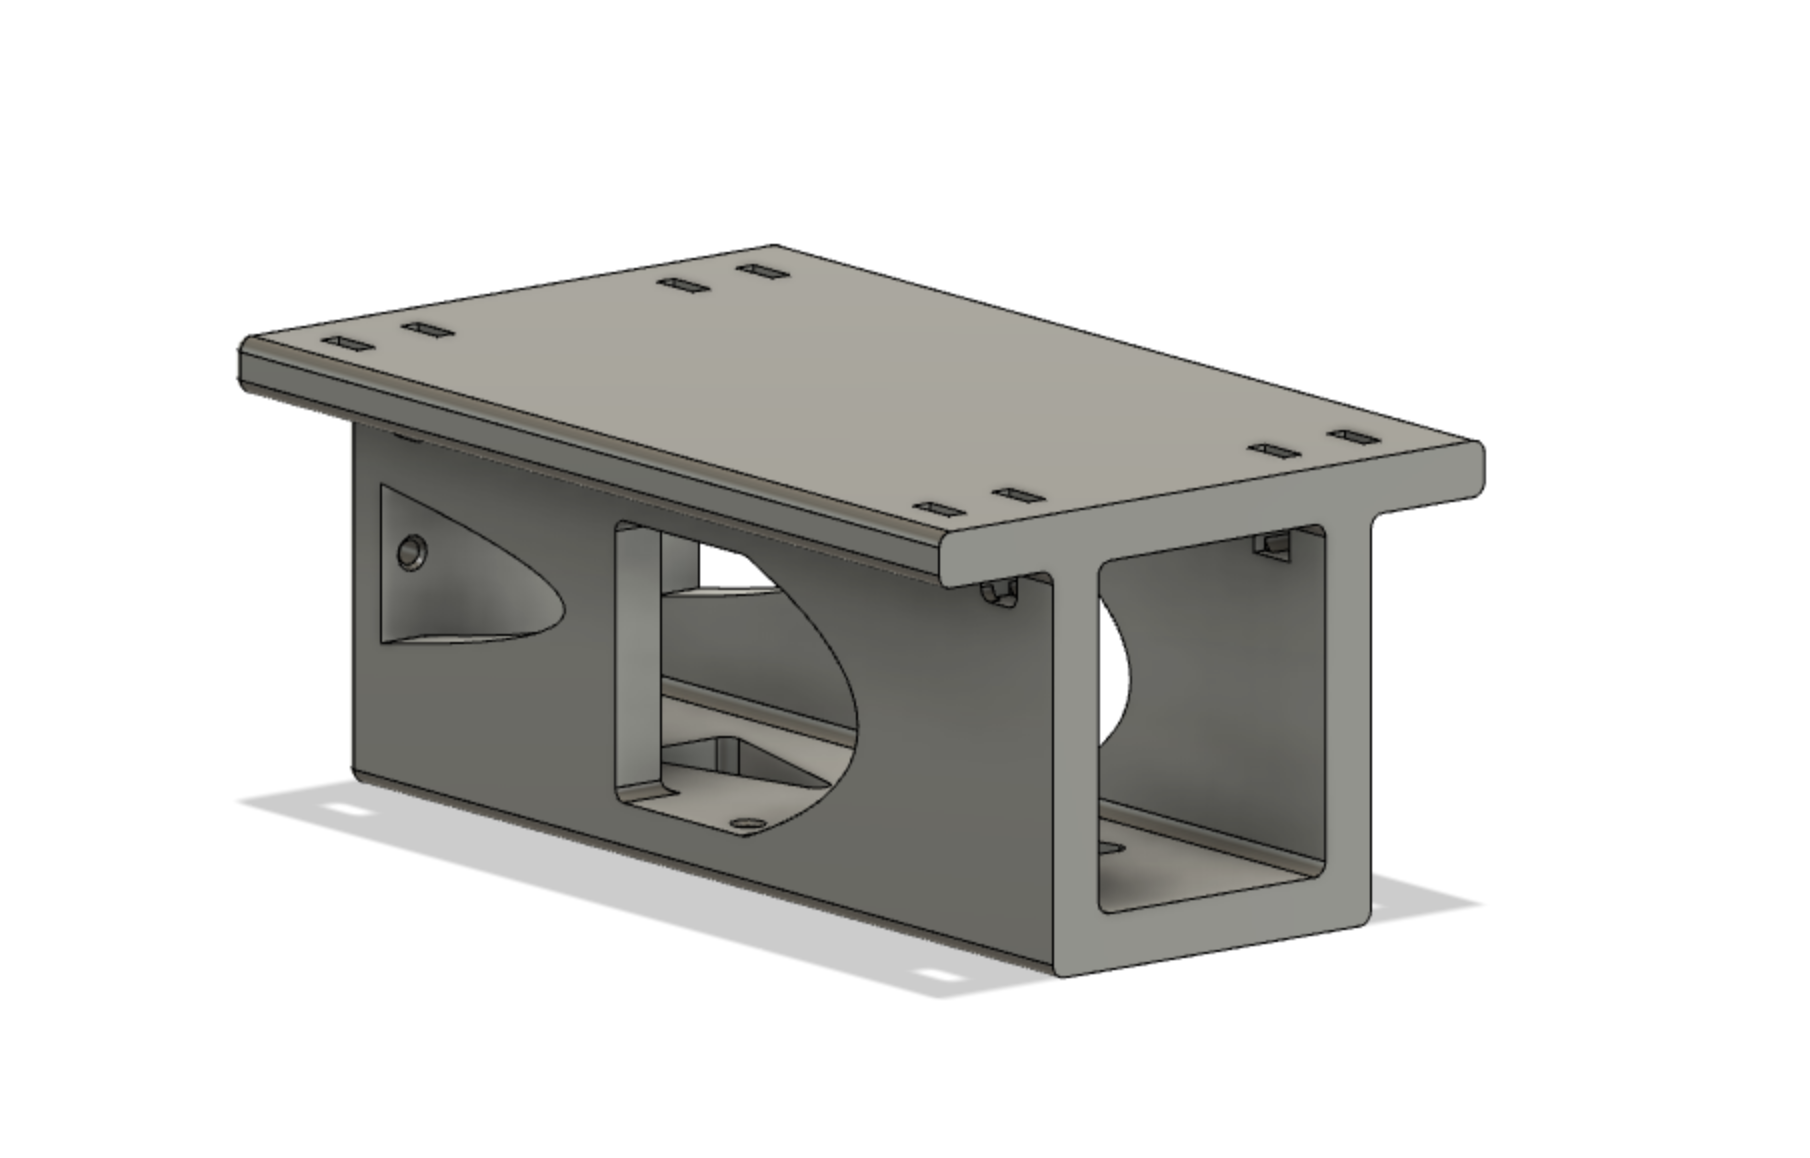
\includegraphics[width=0.9\textwidth]{figs/chapter3/battery-pack.png}
    \caption{Modello CAD del pacco batteria, che funge anche da supporto per la camera inferiore.}
    \label{fig:batpack}
\end{figure}

\begin{figure}
    \centering
    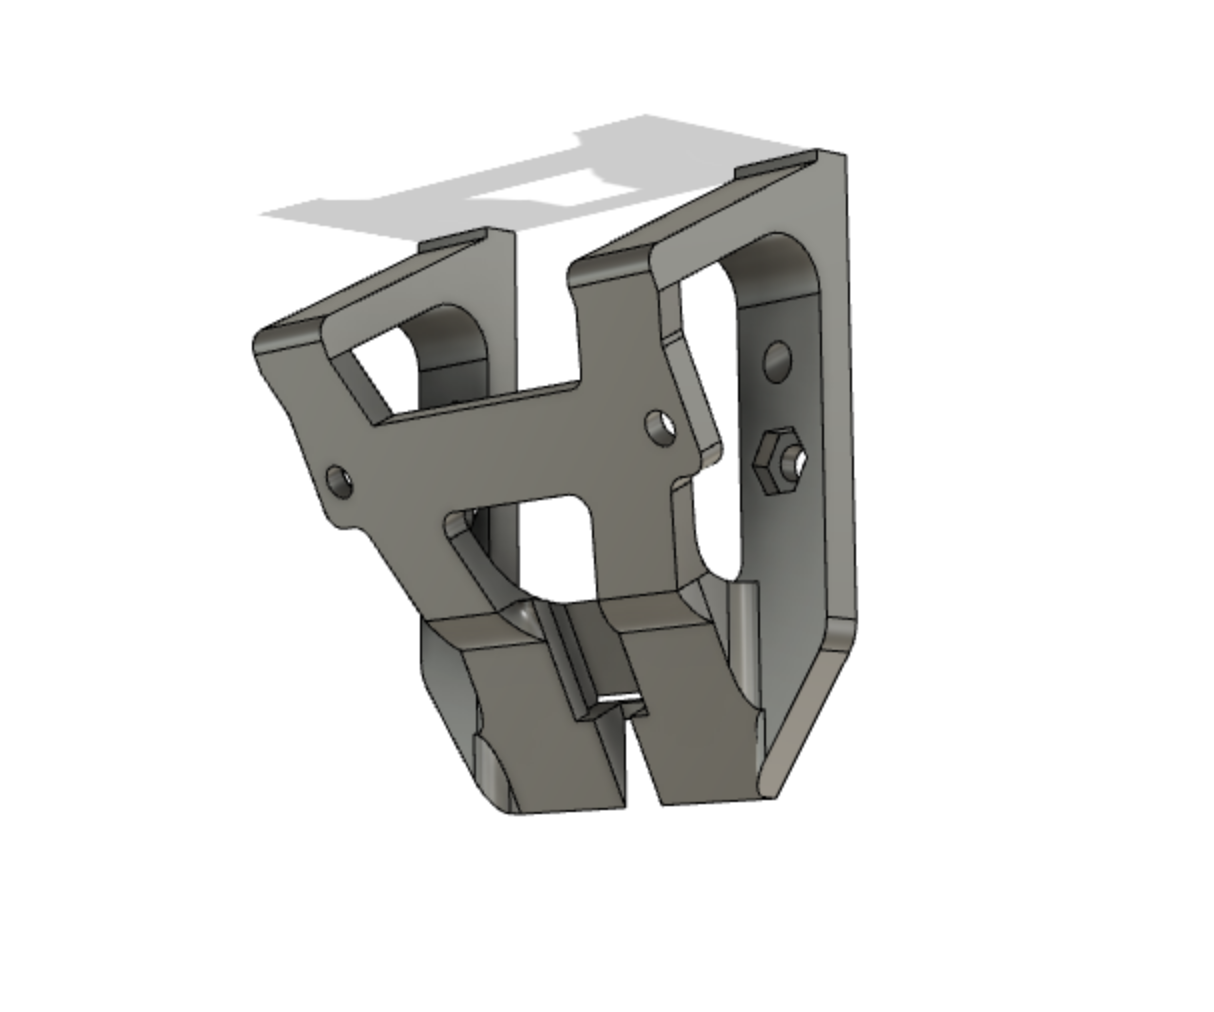
\includegraphics[width=0.9\textwidth]{figs/chapter3/camera-holder.png}
    \caption{Modello CAD del supporto della camera frontale, inclinata verso il basso di 26.6°..}
    \label{fig:frontcam}
\end{figure}

\begin{figure}
    \centering
    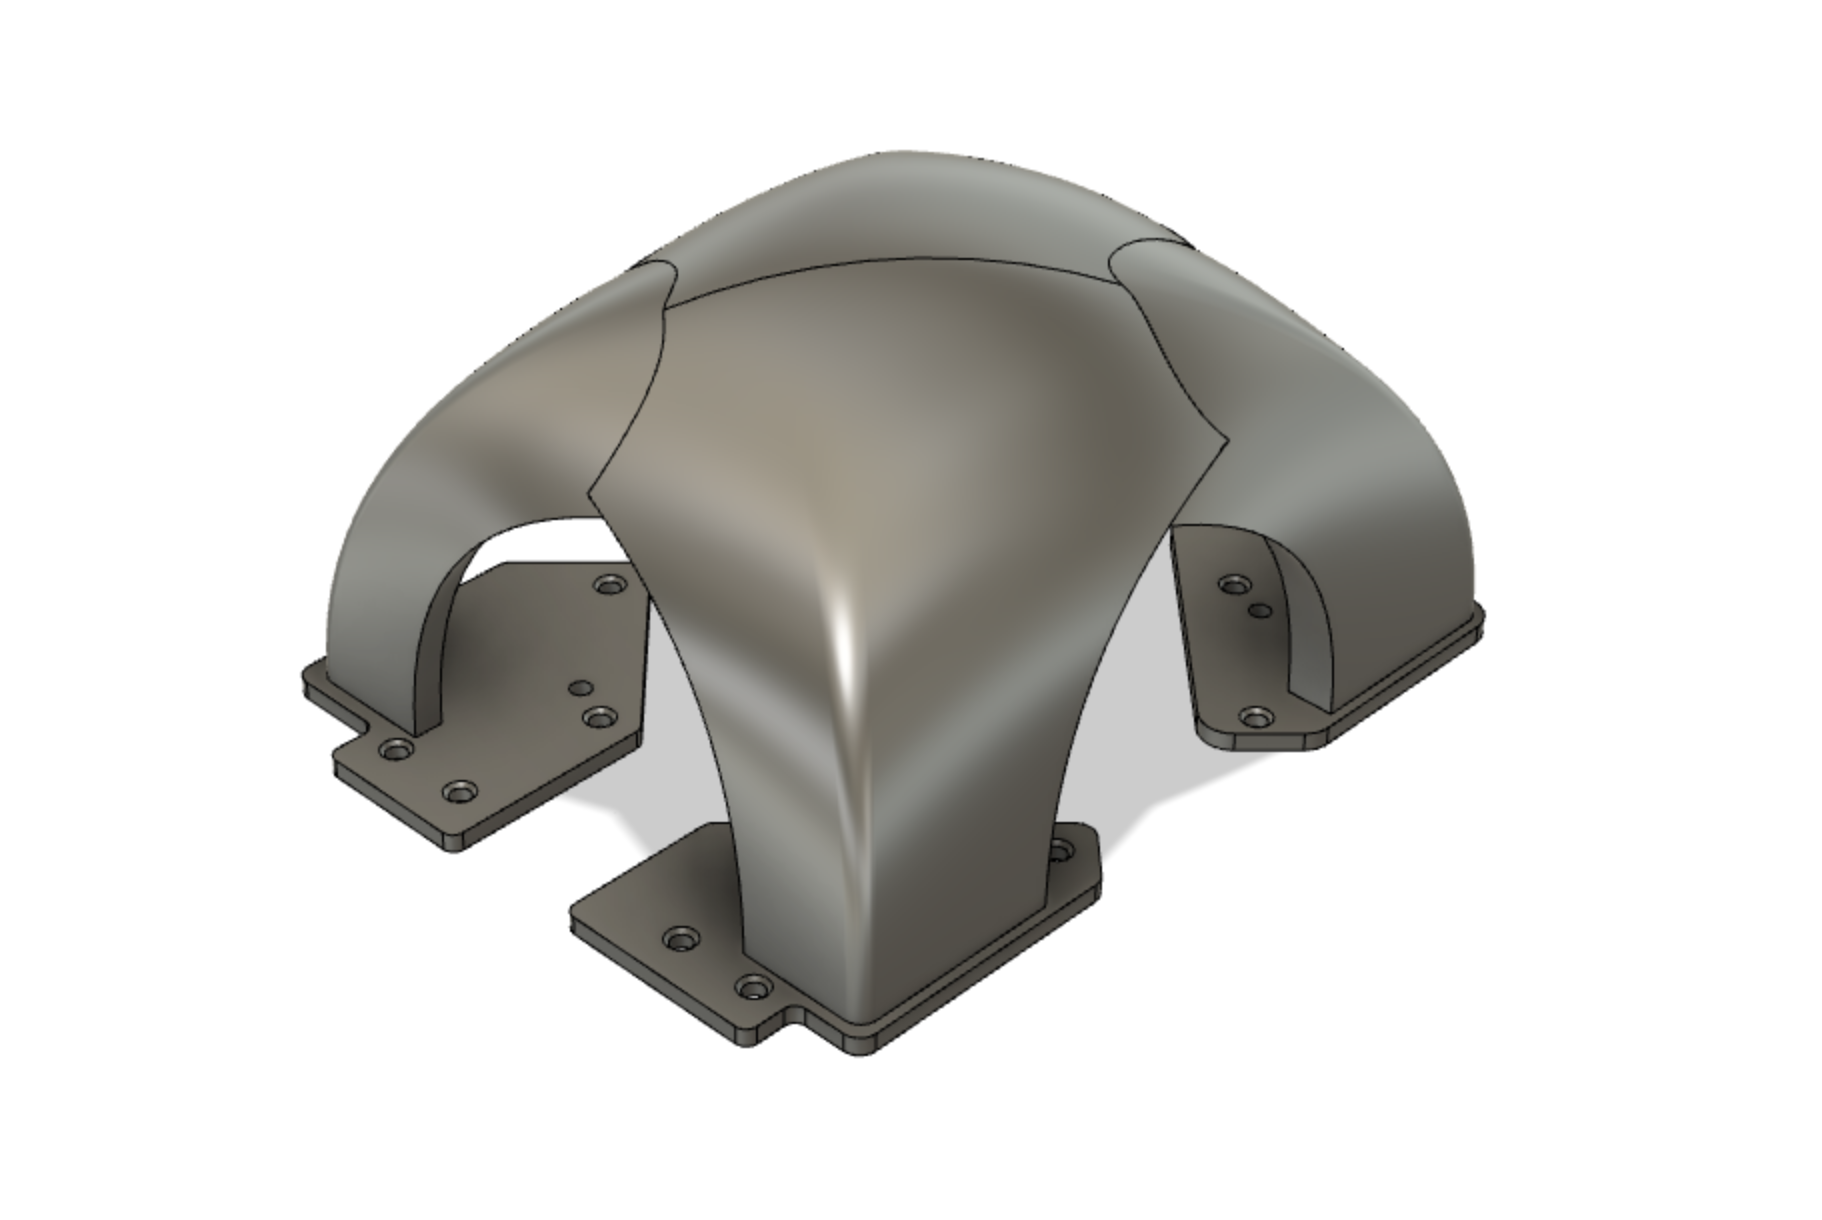
\includegraphics[width=0.9\textwidth]{figs/chapter3/canopy.png}
    \caption{Modello CAD della canopy superiore in TPU, a protezione del computer di bordo.}
    \label{fig:canopy}
\end{figure}

\begin{figure}
    \centering
    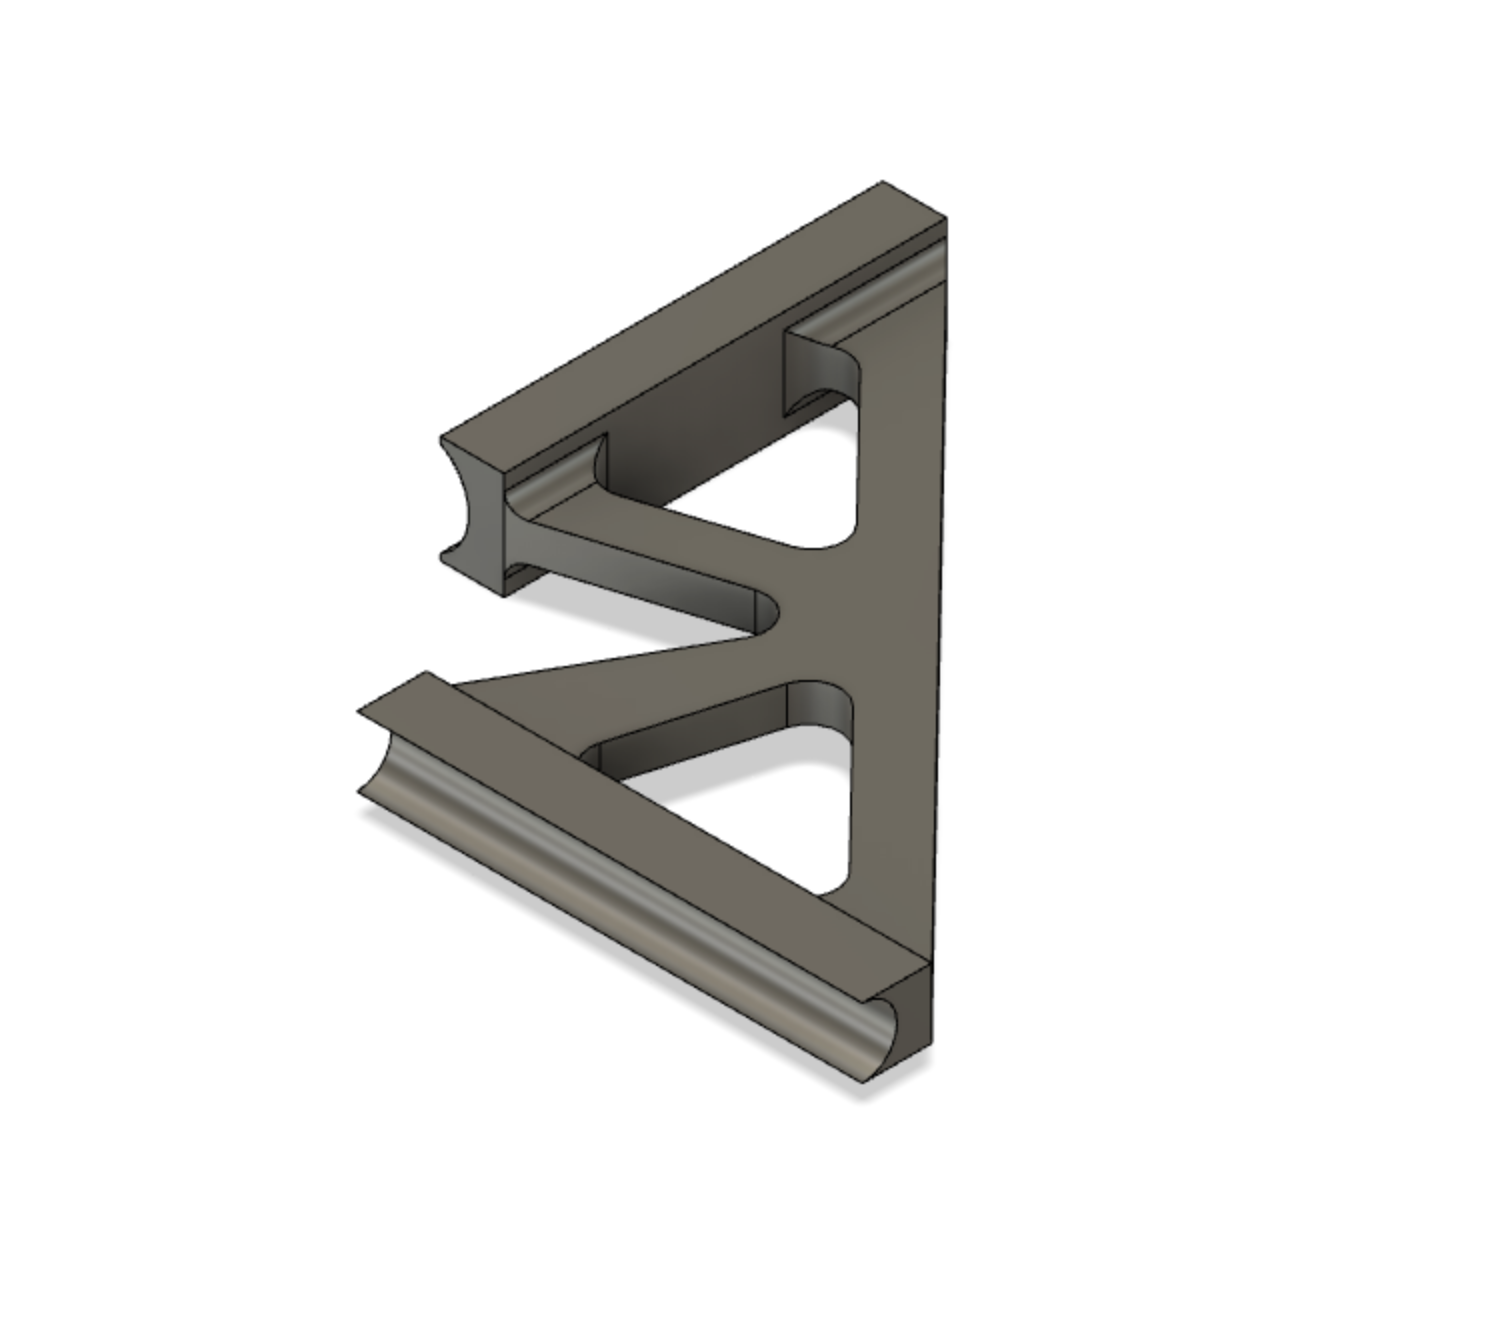
\includegraphics[width=0.9\textwidth]{figs/chapter3/triangle.png}
    \caption{Modello CAD del rinforzo triangolare per i carrelli del frame.}
    \label{fig:triangle}
\end{figure}

\newsection{Operating System}
\indent

\newsection{Software}
\indent

\newsection{Realizzazione}
\indent
